% This is samplepaper.tex, a sample chapter demonstrating the
% LLNCS macro package for Springer Computer Science proceedings;
% Version 2.20 of 2017/10/04
%
\documentclass[runningheads]{llncs}
%
\usepackage{graphicx}
\usepackage{amsmath}
\usepackage{algorithm, algpseudocode}
\graphicspath{{./pics/}}
% Used for displaying a sample figure. If possible, figure files should
% be included in EPS format.
%
% If you use the hyperref package, please uncomment the following line
% to display URLs in blue roman font according to Springer's eBook style:
% \renewcommand\UrlFont{\color{blue}\rmfamily}

\begin{document}
%
\title{Words in Biology}
%
%\titlerunning{Abbreviated paper title}
% If the paper title is too long for the running head, you can set
% an abbreviated paper title here
%
\author{Rahul Kejriwal\inst{1} \and Srinidhi Prabhu\inst{1}}
%
% \authorrunning{F. Author et al.}
% First names are abbreviated in the running head.
% If there are more than two authors, 'et al.' is used.
%
\institute{IIT Madras\\\email{\{cs14b023,cs14b028\}@smail.iitm.ac.in}}
%
\maketitle              % typeset the header of the contribution
%

\begin{abstract}
The objective of this work is to investigate learning of functional units in proteins by applying unsupervised word segmentation techniques from Natural Language Processing literature. The learnt functional units can reveal information regarding the protein like its family, fold, class etc.

\keywords{Unsupervised Word Segmentation \and Description Length \and Protein Classification}
\end{abstract}

\section{Introduction \& Motivation}

Proteins are composed of one or more long chains of amino acids. About 500 amino acids are known but most of them are quite rare. Each amino acid can be encoded by a unique identifier (a unique one or two letter sequence) and hence, each protein can be represented as a string of amino acid identifiers.

This representation parallels natural language (NL) sentences and motivates parallels between the two domains. In particular, we can think of functional units in proteins as subsequences of amino acids that cause the protein to exhibit certain properties. These substrings are analogous to words in a sentence. This motivates the application of word segmentation techniques from NL domains for proteins. 

Word segmentation has been extensively studied in the NL domain and algorithms exist that allow learning of segmentation rules. Although the task of word segmentation is trivial for languages like English that mark the end of words with spaces or punctuations, there are languages like Chinese and Japanese which do not explicitly mark the end of words. Thus, sentences in Chinese and Japanese look like a stream of characters that need to be partitioned into words. This has led to extensive work for automatic segmentation of sentences. 

In particular, a class of this work has been directed along the lines of unsupervised induction of segmentation rules from large text corpora. They do not need any seed knowledge and they learn segmentation rules from unannotated corpora. This allows direct application of these techniques to protein strings.	

This work aims to compare the performance of various unsupervised segmentation algorithms on English text as well as protein strings. We also investigate the task of protein classification. 

\section{Related Work}

Tendulkar et al. \cite{tendulkar2013parallels} have beautifully motivated the parallels between Natural Language and Biology domains. They discuss how proteins and DNA mirror Natural Language sentences. 

Devi et al. \cite{devi2017protein} build on this intuition and investigate the use of Minimum Description Length (MDL) Gain for unsupervised segmentation of proteins and show the effectiveness of this technique in the Protein Classification task. Our work is inspired by this paper and aims to study the performance of different segmentation algorithms. 

Many unsupervised word segmentation techniques have been discussed in the literature. Most of these techniques use MDL-based segmentation \cite{zhikov2013efficient,kitt1999unsupervised,hewlett2011fully,chen2013improved}. We will elaborate on these techniques in subsequent sections.

\section{Segmentation Task}

\subsection{MDL Based Approaches}

Minimum Description Length (MDL) is motivated by Occam's Razor. The belief is that the segmentation that best compresses the string is actually the true segmentation. This works because a language generally has repeating patterns and not all n-grams are equiprobable. For a hypothetical language, where the next character given all the previous characters was equiprobable, MDL based techniques would fail. Redundancy in language is exploited by the MDL paradigm. 
The total description length of the encoded string along with the codebook is used as a metric to discriminate among candidate segmentations. The lower the description length, the better the segmentation. 

Assume the segmented string has segments $w_{i}$ with counts $wc_{i}$. The codebook simply contains all the types of segments that have been learnt. Let the codebook contain $c_{i}$ count of the $i^{th}$ character. Further, let N be the total number of tokens in the segmentation and M be the total number of characters in the codebook. Let $s$ denote a segmentation and $S$ denote the set of all segmentations of a given string. Then,

$$segmentation = argmin_{s \in S}\ \Sigma_{i}\ wc_{i}log(\frac{wc_{i}}{N}) + \Sigma_{j}\  c_{j}log(\frac{c_{j}}{M})$$

This can be thought of as an application of the noisy channel model. The sentence seen arises from an unseen segmented sentence. The segmentation information is lost in the forward process and we observe the unsegmented sentence. The task is to determine the best segmentation that could have given rise to the observed unsegmented sentence. Let the observed sentence be denoted by OS. Thus, 

$$ segmentation = argmax_{s \in S}\ P(OS|s)P(s)$$

The forward process is deterministic and hence, $P(OS|s) = 1$. Thus, the algorithm basically reduces to choosing the segmentation with highest prior probability $P(s)$. Here, we incorporate our intuition regarding MDL and say that the most probable segmentation is that which minimizes the total description length.

\begin{algorithm}
		\caption{Find segmentation of observed sentence}
		\begin{algorithmic}[1]
			\Procedure{FindSegmentation}{$OS$}
			\State $segmentations = GenerateAllSegmentations(OS)$
			\State Return $argmin_{s \in segmentations} DescriptionLength(s)$
			\EndProcedure
		\end{algorithmic}
\end{algorithm}

There are $O(2^n)$ segmentations for a string of length $n$ and it takes $O(n)$ time to compute description length for any given segmentation. The naive algorithm thus has a time complexity of $O(n2^n)$ which is intractable. Typically, $n$ is very large as even small texts contain large number of characters. Practically, algorithms should have complexity atmost $O(n^2logn)$ for tractability.

As exhaustive search is prohibitively expensive, most algorithms are approximate. They constrain the search space using certain heuristics and try to come up with better candidate segmentations. MDL is then used to discriminate among the candidate segmentations. 

Here, we discuss two such approximate algorithms given in \cite{kitt1999unsupervised} and \cite{zhikov2013efficient}.

\subsection{Approach 1: Segmentation using Description Length Gain}

Kit el al. \cite{kitt1999unsupervised} describe a dynamic programming based approximation to the problem of searching for the ideal segmentation. The algorithm is given in Algorithm \ref{dl_gain}. We have tried to be complete in our description of the algorithm but for better explanations, the reader is encouraged to go through \cite{kitt1999unsupervised}.

This algorithm tries to find the ideal segmentation of a string till the $k^{th}$ index. The string $t_0..t_k$ can be segmented as $t_j..t_k$ concatenated to the ideal segmentation of $t_0..t_j$. The algorithm then chooses the value of $j$ that optimizes the Description Length gain criteria. It is essential to note that this is an approximation as the algorithm only makes greedy choices. There is no guarantee that this chosen segmentation is really optimal. DL is a global property and optimality of subproblems does not ensure optimality of the entire problem. Further, for computation of Description length gain, we consider the gains of replacing one string at a time and sum these gains hoping that this will lead us to better \texttt{actual} description length.

While this algorithm does efficiently look at all possible segmentations in the exponential search space, it does not discriminate among all the segmentations using our objective function, i.e., DL, rather it uses an approximate heuristic DL Gain to guide its search.

\begin{figure}[b]
\centering
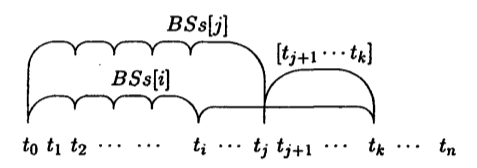
\includegraphics[width=0.6\linewidth]{pics/viterbi_seg.png}
\label{viterbi_seg}
\caption{Dynamic programming view of possible segmentations for $t_0..t_k$. Notice the presence of common subproblems.}
\end{figure}

The complexity of this algorithm is $O(NMVlogN)$ where $N$ is corpus length, $M$ is a bound on the number of prefixes ending at any index having count greater than equal to 2, and $V$ is size of vocabulary. $M$ and $V$ are typically independent of the size of the corpus and may be treated as constants. Thus, the time complexity of this algorithm can be taken as $O(NlogN)$. 

\begin{algorithm}
	\caption{Find Optimal Segmentation using DL Gain paradigm}
	\label{dl_gain}
	\begin{algorithmic}[1]
		\Procedure{OptimalSegmentation}{$U = t_1t_2..t_n$}
        \For{k = 0 to n} 
		    \State $OS[k] = \phi$
            \For{j = k-1 to 0 } 
                \If{$c[t_{j+1}..t_k] < 2$} \State{break} \EndIf 
                \If{$DLG(OS[j] \oplus {[t_{j+1}..t_k]}) > DLG(OS[k])$}
                    \State $OS[k] = OS[j] \oplus \{[t_{j+1}..t_k]\}$
                \EndIf
            \EndFor
        \EndFor
		\State Return $OS[n]$
		\EndProcedure
	\end{algorithmic}
\end{algorithm}

Let $OS$ be a segmentation, i.e., an ordered list of strings that the corpus $X$ has been segmented into. $c(x)$ denotes count of string $x$ in corpus $X$ and $c'(x)$ denotes count of string $x$ in modified corpus after all occurrences of string $r$ in $X$ have been replaced by identifier $s$. $c_s(x)$ denotes count of string $x$ in $s$. $n'$ is the new length of modified corpus. Note that for finding counts $c(x)$ suffix array of the original corpus is used and binary search is done to find the bounds for the substring being counted.
 
\begin{align*}
    DLG(OS[j]) &= \Sigma_{s \in OS[j]}\ DLG(s)  \\
    DLG(s \in X) &= DL(X) - DL(X[r \rightarrow s]\oplus s) \\
    DL(X) &= -\Sigma_{x \in V}\ c(x) log \frac{c(x)}{|X|} \\
    DL(X[r \rightarrow s]\oplus s) &= -\Sigma_{x \in V \cup \{r\}}\ c'(x) log \frac{c'(x)}{n'} \\
\end{align*}
\begin{align*}
    c'(x) &= \left\{
    \begin{array}{ll}
        c(s) & if\ x = r  \\
        c(x)-c(s)c_s(x)+c_s(x)  & otherwise
    \end{array} 
    \right.\\
    n' &= n - c(s)|s| + c(s) + |s| + 1\\
\end{align*}

\subsection{Approach 2: Segmentation using Branching Entropy and MDL}

This approach uses a measure called Branching Entropy. Branching Entropy captures the amount of uncertainty associated with the next character given the previous few characters. The intuition is that typically word endings should have higher uncertainty about next character as compared to internal word characters. 

Formally, branching entropy is given by:

$$H(X_k|x_{k-1},..,x_{k-n}) = - \Sigma_{x \in X} P(x|x_{k-1},..,x_{k-n})log_2 P(X_k|x_{k-1},..,x_{k-n})$$

More generally, the bidirectional version of this formulation is used. This is given by: 
\begin{align*}
    H(X_{k;k-1}|x_{k-1},..,x_{k-n};x_{k},..,x_{k+n-1}) & = -\Sigma_{x \in X} P(x|x_{k-1},..,x_{k-n})log_2 P(X_k|x_{k-1},..,x_{k-n}) \\
    & -\Sigma_{x \in X} P(x|x_{k},..,x_{k+n-1})log_2 P(X_k|x_{k},..,x_{k+n-1}) \\
\end{align*}

The value of $n$ corresponding to the order of the language model is left as a hyperparameter.

This approach has a 3-step process:
\begin{enumerate}
    \item \textbf{Generation of Initial Hypothesis Segmentation:} The algorithm first builds an initial hypothesis segmentation by creating word boundaries at those indices where the branching entropy crosses a threshold value. The authors remark that the distribution of DL w.r.t. this threshold value is actually unimodular. Hence, we can do a modified version of binary search to reach the optimal threshold value. This procedure is given in Algorithm \ref{init_hyp}.
    \item \textbf{Improvement of DL by local modifications:} Next the algorithm tries to improve the DL of the hypothesis segmentation by making local changes to the word segments. It tests whether splitting a token or merging 2 tokens leads to a decrease in DL and accepts the change if it does. These candidate local changes are guided in order by the branching entropy values of the indices. This process is repeated till convergence and is detailed in Algorithm \ref{local_search}.
    \item \textbf{Improvement of DL by global modifications:} Finally, the algorithm tries global level changes to improve DL by trying out global level token splitting or merging. This is guided by the cost of the word segment. This procedure is elaborated in Algorithm \ref{global_search}.
\end{enumerate}

For a more detailed description of the algorithm, the reader is encouraged to go through \cite{zhikov2013efficient}.

Algorithms \ref{local_search} and \ref{global_search} closely model search procedures that are inherently greedy and closely resemble Hill Climbing Search (more appropriately Hill Descending Search). They accept any change in the hypothesis segmentation that improves the value of the objective function, i.e., DL and repeat this until convergence. Hence, they get stuck at local optima. It is important to note that this search is \textbf{not exhaustive} and is guided by heuristics. There is no guarantee that iteratively accepting small changes that lead to improvement in DL will guide us towards the global optima.  

The time complexity of Algorithm \ref{init_hyp} is $O(NVlogN)$, of Algorithm \ref{local_search} is $O(MN^2)$ and that of Algorithm \ref{global_search} is $O(MN^3)$. Please note that these upper bounds are not very tight and are in general pessimistic. Here, $M$ is the bound on the number of iterations till convergence for Algorithm \ref{local_search} and \ref{global_search}. Typically, $M$ is quite low. 

Note that Dynamic Programming has to be used for computing the DL of each hypothesis and suffix arrays have to be used for computing counts of n-grams to achieve these time complexities.

\begin{algorithm}
	\caption{Generate initial hypothesis}
	\label{init_hyp}
	\begin{algorithmic}[1]
        \State thresholds[]= $H(X_k)$ values
        \State threshold = median of thresholds[]
        \State step = length of thresholds[]/4
        \State direction = ascending
        \State minimum = $+\infty$
        \While{$step > 0$}
            \State nextThreshold = thresholds[] value one step in last direction
            \State DL = calculateDL(nextThreshold)
            \If{$DL<minimum$}
                \State minimum = DL
                \State threshold = nextThreshold
                \State step = step / 2
                \State continue
            \EndIf
            \State reverse direction
            \State nextThreshold = thresholds[] value one step in last direction
            \State DL = calculateDL(nextThreshold)
            \If{$DL<minimum$}
                \State minimum = DL
                \State threshold = nextThreshold
                \State step = step / 2
                \State continue
            \EndIf
            \State reverse direction
            \State step = step / 2
        \EndWhile
	\end{algorithmic}
\end{algorithm}

\begin{algorithm}
	\caption{Compress local token co-occurences}
	\label{local_search}
	\begin{algorithmic}[1]
        \State path[] = positions sorted by $H(X_k)$ values
        \State minimum = DL of model produced at initialization
        \Repeat
            \For{i = max $H(X_k)$ to min $H(X_k)$}
                \State pos = path[i]
                \If{no boundary exists at pos}
                    \State leftToken = token to left from pos
                    \State rightToken = token to right from pos 
                    \State longToken = leftToken + rightToken
                    \State calculate DL after splitting
                    \If{$DL < minimum$}
                        \State Accept split, update model, update DL variables
                    \EndIf
                \EndIf
            \EndFor
            \For{i = min $H(X_k)$ to max $H(X_k)$}
                \State pos = path[i]
                \If{boundary exists at pos}
                    \State leftToken = token to left from pos
                    \State rightToken = token to right from pos 
                    \State longToken = leftToken + rightToken
                    \State calculate DL after merging
                    \If{$DL < minimum$}
                        \State Accept merge, update model, update DL variables
                    \EndIf
                \EndIf
            \EndFor
        \Until{no change is evident in model}
	\end{algorithmic}
\end{algorithm}

\begin{algorithm}
	\caption{Lexicon clean-up procedure}
	\label{global_search}
	\begin{algorithmic}[1]
        \State types[] = lexicon types sorted by cost
        \State minimum = DL of model produced by Algorithm \ref{local_search}
        \Repeat
            \For{i = min cost to max cost}
                \For{pos = middle to both ends of types[i]}
                    \State longType = types[i]
                    \State leftType = sequence from first character to pos
                    \State rightType = sequence from pos to last character
                    \State calculate DL after splitting longType into leftType and rightType
                    \If{$DL < minimum$}
                        \State accept split, update model, update DP variables
                        \State break out of inner loop
                    \EndIf
                \EndFor
            \EndFor
            \State types[] = lexicon types sorted by cost
            \For{i = max cost to min cost}
                \For{pos = middle to both ends of types[i]}
                    \State longType = types[i]
                    \State leftType = sequence from first character to pos
                    \State rightType = sequence from pos to last character
                    \State calculate DL after merging longType into leftType and rightType
                    \If{$DL < minimum$}
                        \State accept merge, update model, update DP variables
                        \State break out of inner loop
                    \EndIf
                \EndFor
            \EndFor
            \State types[] = lexicon types sorted by cost
        \Until{no change is evident in model}
	\end{algorithmic}
\end{algorithm}

\subsection{Approach 3: Segmentation as Search}

The problem of segmentation can also modeled as a search problem. We can model it as a problem of searching for the correct or best segmentation in the space of possible segmentations. When the search space is exponential in the number of input variables, we use AI search techniques to come up with good (maybe not optimal) solutions to the problem. We can use similar search techniques to hopefully come up with good segmentations in this case.

We attempt to search for good segmentations by using a Genetic Algorithm(GA) that searches in the space of segmentations. We define the components of the algorithm as given below:
\begin{enumerate}
    \item \textbf{Fitness Function:} The fitness function is the negative of the Description Length(DL). We wish to maximize the fitness function.
    \item \textbf{Representation of an individual:} An individual is represented as a list of indices at which it segments the string.
    \item \textbf{Crossover operation:} Given two individuals I$_1$ and I$_2$, we choose random indices to split the two individuals. The first part of I$_1$ is concatenated with the second part of I$_2$ and the first part of I$_2$ is concatenated with the second part of I$_1$. We remove the duplicate indices in the lists and then perform a merge operation over the two parts to generate the crossed individuals.
    \item \textbf{Mutation:} Remove an index from an individual or insert an index (not already in the list) into the individual, with equal probability. 
\end{enumerate}

%\subsection{Non-MDL Based Approaches}
%Identifying segments based on MDL are not the only methods to identify segmentation. This section describes non-MDL based methods towards segmentation. The first method is specific to the protein domain and uses domain knowledge to generate words in protein sequences. The second method models the segmentation procedure as a search problem.


\subsection{Experiments}

The word segmentation algorithms were applied to English text and we measured precision and recall of the word boundaries detected. Note that since we do not have an annotated corpus with word segmentation, we have made a simplifying assumption that all words are segmented at the space character. Using this assumption, we have annotated our corpus and computed the precision and recall of the segmentation algorithm. 

For Approach 1 and 2, we ran the segmentation algorithms on the text (first 75000 characters) 'Alice in Wonderland' present as part of  nltk.corpus.gutenberg. 

For Approach 3, we ran the GA over a corpus with about 1700 characters. We tried out the GA for different sizes of population (varying from 10 to 1000) and different number of iterations (varying from 10 to 1000).

\section{Protein Classification}

%\subsection{Approach 1: Classification using learnt functional units}

\subsection{Approach 1: Classification using Deep Learning techniques}

Proteins are inherently sequential in nature and the task of protein classification thus motivates the use of recurrent neural networks. We first learn a vector embedding for each amino acid constituent of the protein and we use this embedded sequence as input to  a Long Short Term Memory Recurrent Neural Network (LSTM RNN). The LSTM RNN computes a vector representation of the protein sequence. Then, a feedforward neural network is trained to predict the class of the protein from the learnt representation of the protein.

LSTMs are widely used deep learning models for sequences and their explanation is beyond the scope of this work. 


\subsection{Approach 2: Dictionary-based Segmentation}
For segmentation of proteins into words, we first need to identify a measure to evaluate the segmentations. In case of a language like English. the true segmentations are generally known. However, in the case of proteins, the true segmentations are not known. Devi et al. \cite{devi2017protein} specify an extrinsic measure to evaluate the segmentations. They use an MDL-based classifier to classify proteins after they have been segmented. The weighted average precisions and recalls across the classes are used as a mesaure to evaluate the performance of the segmentation.

Yang et al. \cite{yang2008classification} describe a method to classify proteins into classes using a dictionary-based segmentation. We implemented the method described in \cite{yang2008classification} to identify and evaluate segmentations over proteins.

The steps in the segmentation and evaluation are as follows:
\begin{enumerate}
    \item \textbf{Dictionary Building:} The set of 20 amino acids along with a certain number of meaningful $k$-mers ($k$ length sequences of amino acids) are selected and stored in a dictionary. We make an assumption that the words in the protein sequences always belong to the dictionary.
    \item \textbf{Segmentation:} A segmentation algorithm is used to segment the protein sequences.
    \item \textbf{Feature Extraction:} Features are extracted from the segmented proteins, to be used later for classification.
    \item \textbf{Classification:} A classifier is trained over a training set and then tested over a test set.
\end{enumerate}

\textbf{Dictionary Building:} For natural languages, we generally have a predefined set of words in a dictionary. However, we do not have any such set of words given to us in the protein domain. MDL-based approaches are unsupervised approaches to identify words in proteins. In this method, we describe a method to build the dictionary and then identify words. 

We use statistical methods to identify words that are to be put in the dictionary. The steps in dictionary building are given below:
\begin{enumerate}
    \item A maximum word length $MaxLen$ is set. For the case of proteins, this value is set to 4. This value has been obtained from experiments performed by Yang et al. \cite{yang2008classification}. It is further reinforced by facts from biology that specify that four is the typical distance between local interactions among amino acids.
    \item Use some statistical measures to identify words from the given set of proteins. Some of the commonly used statistical measures are:
    \begin{itemize}
        \item \textbf{Frequency:} The substrings that occur most frequently are stored as words in the dictionary.
        \item \textbf{tf-idf:} This criterion not only looks at the frequency of the substrings but also takes into account the distribution of the k-mer across all sequences in the training set. This method is mainly used to identify features for classification of proteins.
    \end{itemize}
\end{enumerate}
For our purpose, we use the most frequent k-mers to identify words to be stored in the dictionary. Currently, we choose all 1-length amino acids. For greater lengths (from 2 to 4), we take the 100 most frequent substrings as the words.

\textbf{Segmentation:} We use a Dynamic Programming based solution to find the optimal segmentation of the protein given the words in the dictionary. The optimal segmentation is one that has the least number of words after segmentation. If there are multiple such segmentations, the one with the largest weight is chosen. The weight of a segmentation is the sum of log occurrences of each word in the training corpus. The details of the segmentation procedure are described in Algorithm~\ref{alg:segment}. The algorithm is adapted from \cite{yang2008classification}.

% Write algo here
\begin{algorithm}[h!]
\caption{Search Segmentation}
\label{alg:segment}
\begin{algorithmic}[1]
\Procedure{Search}{$D, S, p$} // $D$ is the dictionary, $S$ is the string and $p$ is the position 
\State $segNum$ and $wordLen$ are two global arrays of size N, where N is the length of the string. $segNum$ stores the number of segments and $wordLen$ stores the length of the word segmented.
    \If{$p = N$}
        \State $segNum_p \gets 1, wordLen_p \gets 1$
        \State \Return $segNum_p$
    \EndIf
    \If{$segNum_p \neq 0$}
        \State \Return $segNum_p$ // The position has been visited 
    \EndIf
    \State Initialize $len$ and $num$ to zero arrays with a maximum size of $maxLen$.
    \For{$k\ =\ 1\ to\ maxLen$}
        \If{k-mer beginning from $p$ $\in\ D$ }
            \State $len_k \gets k$
            \State $num_{k} = 1\ +\ Search(D, S, p+k)$
        \EndIf
    \EndFor
    \If{Multiple segmentation ways have the same least number of segments}
        \State Calculate weight product for each segmentation which has the least segments.
    \EndIf
    \State $wordLen_p \gets len_k$, $segNum_p \gets num_k$, where the kth segmentation way has the maximum weight product.
    \State \Return $segNum_p$
  
\EndProcedure
\end{algorithmic}
\end{algorithm}

\subsection{Experiments}

\textbf{LSTM RNN based classification}

\textbf{Feature Extraction:} The amino acid constituents are encoded using one-hot vectors and fed as is to the LSTM network. No explicit feature extraction is done.

\textbf{Classification:} A neural network based classifier is trained on the LSTM hidden representation of the proteins. 24,558 proteins were used in training and the results are reported over a test set consisting of 5,049 proteins.
\ \\ \newline

\noindent \textbf{Dictionary-based segmentation and classification}

%Put feature extraction and classification in experiments?
\textbf{Feature Extraction:} We use a vector-space kind of model with bag-of-words assumption to represent the segmented protein sequences as features. So, each word in the dictionary is a feature and the number of occurrences of the word in a given protein gives the weight of the feature.

\textbf{Classification:} We use the SVM classifier with RBF kernel for classification. The classifier is trained over 24,558 proteins and the results are reported over a test set consisting of 5,049 proteins.


\section{Results}

\subsection{Word Segmentation}

We report the precision and recall of the segmentation algorithms over the test corpus here. 

\begin{table}[H]
\centering
\begin{tabular}{ c | c c c}\hline
\textbf{Approach} & \textbf{Precision} & \textbf{Recall} & \textbf{F1-score} \\ \hline
Approach 1 & 0.445 & 0.884 & 0.592 \\ 
Approach 2 & 0.564 & 0.832 & 0.673 \\ 
\end{tabular}
\caption{Performance metrics of word segmentation algorithms}
\label{tab:perf_word_seg}
\end{table}
For the case of genetic algorithms, we do not observe any useful results. We observe that the algorithm merges the entire text into a single segment for most cases. 

\subsection{Protein Classification}
We report our results for protein classification on the SCOPe dataset. This dataset contains proteins belonging to 4 classes. The results for classification of proteins using RNNs is given in Table~\ref{tab:rnn_res}.
\begin{table}[H]
\centering
\begin{tabular}{| c| c| c| c|}\hline
\textbf{Class} & \textbf{Precision} & \textbf{Recall} & \textbf{F1-score} \\ \hline
0 & 0.90 & 0.92 & 0.91 \\ \hline
1 & 0.94 & 0.87 & 0.90\\ \hline
2 & 0.93 & 0.92 & 0.92 \\ \hline
3 & 0.78 & 0.85 & 0.82 \\ \hline
Average & 0.89 & 0.89 & 0.89 \\ \hline
\end{tabular}
\caption{Results of protein classification using RNNs}
\label{tab:rnn_res}
\end{table}

The results for classification of proteins using the dictionary-based approach are given in Table~\ref{tab:dict_res}.
\begin{table}[H]
\centering
\begin{tabular}{| c| c| c| c|}\hline
\textbf{Class} & \textbf{Precision} & \textbf{Recall} & \textbf{F1-score} \\ \hline
0 & 0.71 & 0.76 & 0.73 \\ \hline
1 & 0.80 & 0.76 & 0.78 \\ \hline
2 & 0.81 & 0.83 & 0.82 \\ \hline
3 & 0.64 & 0.62 & 0.83 \\ \hline
Average & 0.75 & 0.75 & 0.75 \\ \hline
\end{tabular}
\caption{Results of protein classification using dictionary}
\label{tab:dict_res}
\end{table}

An interesting point to note here is that we achieve an average precision and recall of 75\% on classification by using a naive vector space model. The RNN-based classifier outperforms the naive vector space model (as expected). It achieves about 89\% average precision and recall on classification. 



\section{Future Work}
\begin{enumerate}
    \item When we use GAs for segmentation of English, we can use constraints like size of a word can't be greater than 15. These can help in guiding the search to better segmentations.
    \item One could use a language model to classify segmented proteins. We can think of each class of protein as having its own language. The protein is classified into the class that best models the segmentation.
    \item We could extend our approaches to evaluate our methods on the proteins domain.
\end{enumerate}




%
% ---- Bibliography ----
%
% BibTeX users should specify bibliography style 'splncs04'.
% References will then be sorted and formatted in the correct style.
%

\bibliography{ref}
\bibliographystyle{splncs04}

\end{document}
